%%%%%%%%%%%%%%%%%%%%%%%%%%%%%%%%%%%%%%%%%
% Beamer Presentation
% LaTeX Template
% Version 1.0 (10/11/12)
%
% This template has been downloaded from:
% http://www.LaTeXTemplates.com
%
% License:
% CC BY-NC-SA 3.0 (http://creativecommons.org/licenses/by-nc-sa/3.0/)
%
%%%%%%%%%%%%%%%%%%%%%%%%%%%%%%%%%%%%%%%%%

%----------------------------------------------------------------------------------------
%	PACKAGES AND THEMES
%----------------------------------------------------------------------------------------

%\documentclass{beamer}
\documentclass[12pt, aspectratio=169]{beamer}
\usepackage{keynote-portfolio}

\mode<presentation> {

% The Beamer class comes with a number of default slide themes
% which change the colors and layouts of slides. Below this is a list
% of all the themes, uncomment each in turn to see what they look like.

%\usetheme{default}
%\usetheme{AnnArbor}
%\usetheme{Antibes}
%\usetheme{Bergen}
%\usetheme{Berkeley}
%\usetheme{Berlin}
%\usetheme{Boadilla}
%\usetheme{CambridgeUS}
%\usetheme{Copenhagen}
%\usetheme{Darmstadt}
%\usetheme{Dresden}
%\usetheme{Frankfurt}
%\usetheme{Goettingen}
%\usetheme{Hannover}
%\usetheme{Ilmenau}
%\usetheme{JuanLesPins}
%\usetheme{Luebeck}
%\usetheme{Madrid}
%\usetheme{Malmoe}
%\usetheme{Marburg}
%\usetheme{Montpellier}
%\usetheme{PaloAlto}
%\usetheme{Pittsburgh}
%\usetheme{Rochester}
%\usetheme{Singapore}
%\usetheme{Szeged}
%\usetheme{Warsaw}

% As well as themes, the Beamer class has a number of color themes
% for any slide theme. Uncomment each of these in turn to see how it
% changes the colors of your current slide theme.

%\usecolortheme{albatross}
%\usecolortheme{beaver}
%\usecolortheme{beetle}
%\usecolortheme{crane}
%\usecolortheme{dolphin}
%\usecolortheme{dove}
%\usecolortheme{fly}
%\usecolortheme{lily}
%\usecolortheme{orchid}
%\usecolortheme{rose}
%\usecolortheme{seagull}
%\usecolortheme{seahorse}
%\usecolortheme{whale}
%\usecolortheme{wolverine}

%\setbeamertemplate{footline} % To remove the footer line in all slides uncomment this line
%\setbeamertemplate{footline}[page number] % To replace the footer line in all slides with a simple slide count uncomment this line

%\setbeamertemplate{navigation symbols}{} % To remove the navigation symbols from the bottom of all slides uncomment this line
}

\usepackage{graphicx} % Allows including images
\usepackage{booktabs} % Allows the use of \toprule, \midrule and \bottomrule in tables

%----------------------------------------------------------------------------------------
%	TITLE PAGE
%----------------------------------------------------------------------------------------

\title[Robot dream]{Robot dream: why do robots sleep?} % The short title appears at the bottom of every slide, the full title is only on the title page

\author{Max Talanov} 
\institute[ITIS: KFU] % Your institution as it will appear on the bottom of every slide, may be shorthand to save space
{
Intellectual robotics department, ITIS \\ % Your institution for the title page
\medskip
\textit{max.talanov@gmail.com} % Your email address
}
\date{\today} % Date, can be changed to a custom date

\begin{document}

\begin{frame}
\titlepage % Print the title page as the first slide
\end{frame}


%----------------------------------------------------------------------------------------
%	PRESENTATION SLIDES
%----------------------------------------------------------------------------------------

%------------------------------------------------
\section{The problem} % Sections can be created in order to organize your presentation into discrete blocks, all sections and subsections are automatically printed in the table of contents as an overview of the talk
%------------------------------------------------
%------------------------------------------------

\begin{frame}
\frametitle{Consciousness $\Rightarrow$ Emotions}
\begin{columns}[c] % The "c" option specifies centered vertical alignment while the "t" option is used for top vertical alignment

\column{.45\textwidth} % Left column and width
\textbf{Human:}
\begin{itemize}
\item Cognition $\Rightarrow$ Consciousness $\Rightarrow$ Emotions
\end{itemize}

\textbf{Machine:}
\begin{itemize}
\item Cognition $\Rightarrow$ Consciousness $\Rightarrow$ Emotions
\end{itemize}

\column{.6\textwidth} % Right column and width
%------------------------------------------------
\begin{figure}
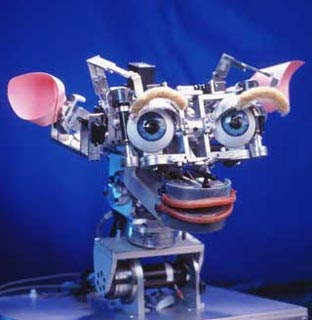
\includegraphics[width=0.8\linewidth]{Kismet_312}
\end{figure}
%------------------------------------------------
\end{columns}
\end{frame}

%------------------------------------------------

\begin{frame}
\frametitle{Robot emotions}
\begin{columns}[c] % The "c" option specifies centered vertical alignment while the "t" option is used for top vertical alignment

\column{.45\textwidth} % Left column and width
\begin{itemize}
\item Biologically plausible
\item Updated cube of emotions by Hugo L\"{o}vheim
\item Implementation: Realistic Neural Network (rNN) 
\end{itemize}


\column{.6\textwidth} % Right column and width
%------------------------------------------------
\begin{figure}
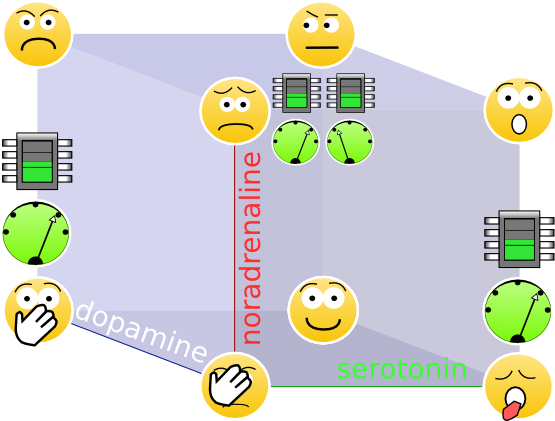
\includegraphics[width=1.0\linewidth]{cube_of_emotional_parameters_machine}
\end{figure}
%------------------------------------------------
\end{columns}
\end{frame}

%------------------------------------------------

\begin{frame}
\frametitle{Machine emotions}
\begin{figure}
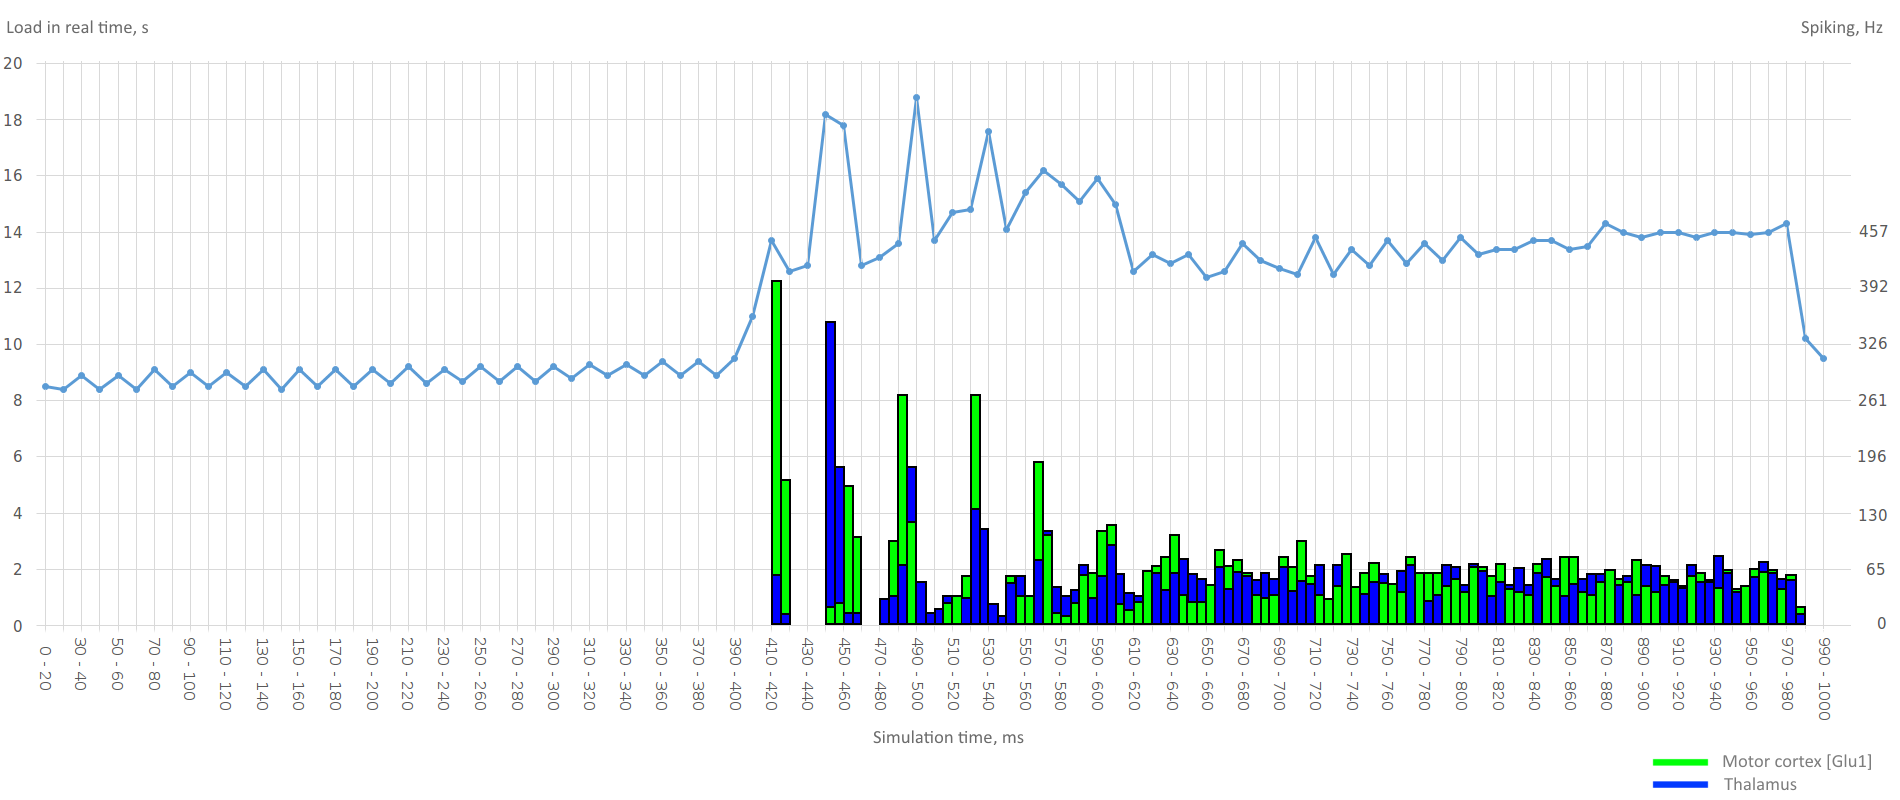
\includegraphics[width=0.99\linewidth]{resultBIG}
\end{figure}
\end{frame}


%------------------------------------------------

\begin{frame}
\frametitle{Robot performance}
\begin{columns}[c] % The "c" option specifies centered vertical alignment while the "t" option is used for top vertical alignment

\column{.45\textwidth} % Left column and width
\begin{itemize}
\item \textbf{AR-601}: Intel Core i7-4700EQ; 8 GB;
\item \textbf{REEM-C}: Intel Core i7 2710QE x 2;
\item \textbf{Nao}: Intel Atom @ 1.6 GHz;
\item \textbf{iCub}: Intel® Core™2 Duo; 2 GB;
\end{itemize}


\column{.6\textwidth} % Right column and width
%------------------------------------------------
\begin{figure}
\includegraphics[width=1.0\linewidth]{ASIMO_Conducting}
\end{figure}
%------------------------------------------------
\end{columns}
\end{frame}

%------------------------------------------------

\begin{frame}
\frametitle{Performance}
\begin{columns}[c] % The "c" option specifies centered vertical alignment while the "t" option is used for top vertical alignment

\column{.45\textwidth} % Left column and width
\textbf{RIKEN} 2013: 1\% of human brain - 250 K-supercomputers
(96 computing nodes, 2.0 GHz 8-core SPARC64; 16 GB of memory), slower than human brain in 1000 times. 

\textbf{Human brain project}: a whole human brain -- 10 exaflop.


\column{.6\textwidth} % Right column and width
%------------------------------------------------
\begin{figure}
\includegraphics[width=1.0\linewidth]{RIKEN_AICS}
\end{figure}
%------------------------------------------------
\end{columns}
\end{frame}


%------------------------------------------------
\section{Solution}
%------------------------------------------------

\begin{frame}
\frametitle{Approach}
\begin{figure}
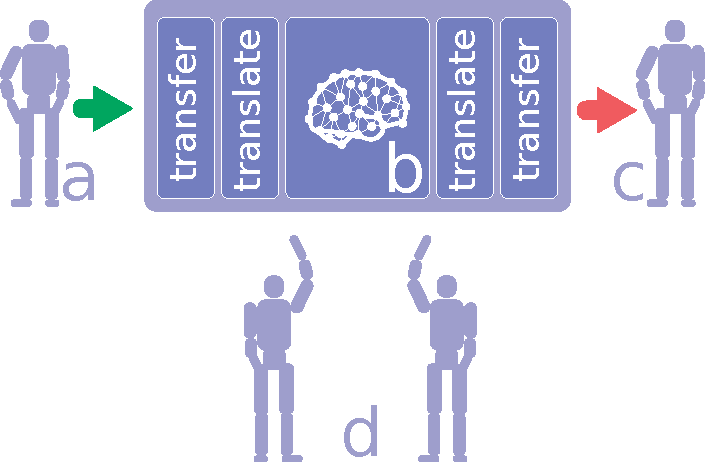
\includegraphics[width=0.8\linewidth]{robot-dream}
\end{figure}
\end{frame}

%------------------------------------------------

\begin{frame}
\frametitle{Day and night phases}

\begin{enumerate}
  \item[a.] A robotic system transfers the accumulated experience into the ``Sleeping brain''.
  \item[b.] Processing:
      \begin{enumerate}
      \item The accumulated experience is transferred from a robotic system to the ``Sleeping brain'';
      \item Simulation starts producing a set of updated rules;
      \end{enumerate}
  \item[c.] The updated rules of the ``Sleeping brain'' are transferred to the robotic system and applied to it.
  \item[d.] The robotic system continues it's job running updated with adjusted emotional reactions and accumulating new experience to be processed again starting from \textbf{A}.
  \end{enumerate}

\end{frame}

%------------------------------------------------

\begin{frame}
\frametitle{Problems and future work}
\begin{itemize}
 \item Robot platform (we started from automatic vacuum cleaner)
 \item Forward translation: rules $\rightarrow$ rNN: ``Pain and Pleasure'' problem
 \item Reverse translation: rNN $\rightarrow$ rules: ``Criteria'' problem
\end{itemize}
\end{frame}

%------------------------------------------------

\begin{frame}
\frametitle{Thank you}

\begin{itemize}
\item Wang, P.: The assumptions on knowledge and resources in models of rationality. Int. J. Mach. Conscious. 3(1), 193–218 (2011)
\item L\"{o}vheim, H. (2012). A new three-dimensional model for emo- tions and monoamine neurotransmitters,
\item Damasio, A. (1999). The Feeling of What Happens.
\item Minsky, M. (2006). The Emotion Machine: Commonsense Thinking, Artificial Intelligence, and the Future of the Human Mind
\item R.W. Picard (2001), "What Does it Mean for a Computer to "Have" Emotions?", Chapter in "Emotions in Humans and Artifacts" 
\end{itemize}

\end{frame}

%------------------------------------------------

\end{document} 
